\documentclass{article}

\usepackage{graphicx} % Allows including images
\usepackage{stackengine}
\usepackage{scalerel}
\usepackage{xcolor}
\usepackage{geometry}
\usepackage{multicol}
\usepackage{listings}

\graphicspath{{./../img/}}
\renewcommand{\abstractname}{}
\renewcommand{\tt}[1]{\texttt{#1}}

\newcommand\dangersign[1][2ex]{%
  \renewcommand\stacktype{L}%
  \scaleto{\stackon[1.3pt]{\color{red}$\triangle$}{\tiny !}}{#1}%
}

\newcommand{\warn}[1]{\begin{center}
\begin{tabular}{ c  p{12cm} }
\dangersign[22pt] & \vspace{-0.6cm} #1
\end{tabular}
\end{center}}

\geometry{
 a4paper,
 left=30mm,
 right=30mm,
 top=30mm,
 bottom=30mm
 }

\lstset{language=Python,
		commentstyle=\color{gray},
		keywordstyle=\color{blue},
		numberstyle=\color{yellow},
		stringstyle=\color{purple}
}


\title{\texttt{theia} \\ \quad \\A 3D Gaussian beam tracer \\ \quad \\ \begin{small} Version 0.1.0 \end{small} \\ \quad \\ \textit{User Guide}}

\author{Rapha\"el Duque}

\begin{document}

\maketitle

\begin{abstract}
theia is a command line program and Python library for 3D Gaussian beam tracing. It supports many different types of optical components, general 3D placing and orientation of these components and general astigmatic Gaussian beams, among other features. theia was developed at the Optics Group of the Virgo gravitational observatory in Cascina, Italy. Please see the \tt{README.md} file of \tt{theia} or surf to \tt{http://37.117.61.221:56000} for more information.

This document is a user's guide to the \texttt{theia} command line tool. It gives the information concerning the installation instructions, the usage and the input and output of \texttt{theia} necessary to operate the program from the command line. For details on the \texttt{theia} Python library, please refer to the API Guide provided along with this User Guide.
\end{abstract}


\tableofcontents
\newpage

\part{Theia User Guide}
\section{\texttt{theia} Quick Start}
For a quick start of theia once you are in the project repository, install theia locally with \texttt{make install}. The command \tt{theia} will then be available to you everywhere and  you can run the tutorial input files (with extension \texttt{.tia}) found in the \texttt{tutos/} folder with \texttt{theia FNAME.tia}, replacing \texttt{FNAME.tia} by one of the tutorial files.

The input \tt{.tia} files provide (among other things) the optical setup information in text form. The output \tt{.out} file reports the physical data (waist position relatively to the origin of the beam and waist size) of the beams generated by the propagation of the input beam.

The \tt{alloptics.tia} tutorial file is particularly fit to quickly learn the input format because all the possible types of optics are used in the corresponding simulation. 

\section{Description of theia}
In the section, we will briefly explain the ideas behind the development of theia, describe the way theia sees the physical objects it deals with and tracing algorithm it implements.

\subsection{The theia rationale}
theia has been designed for flexible and practical operation. This why theia is not only a command line tool, but also a Python library aiming at scripting and written accordingly -- please see the theia API Guide for more details on this library. 

The theia command line tool has it its own right been designed with flexibility and pragmatism in mind. The theia input and output files were thought to allow high level features to insure ease of writing and reading by humans, to be printed out, brought to the optical bench and used as references to follow the evolution of the optical layout and its components, to be read as structured files containing figures one can readily compare to experimental data, etc.

Aiming for flexibility also implies liberty for the user when it comes to input. The theia user can specify as much information as she or he wishes. From specifying zero parameters and using default values for all the arguments to using built-in values such as handy units, users have a large radius of action for their input.

With liberty must also come caution. If the user specifies geometrically inconsistent parameters -- leading to self-intersecting surfaces for instance --, then warnings may be issued to standard output (unless specific command line flags are used, see 3.2) but the simulation will carry on almost unseemingly, and may lead to unexpected behavior. 

\subsection{The operation of theia}
theia is a command line 3D Gaussian beam tracing program. During its operation, input beams and an optical setup are read from an input text file and these beams are traced and interact with optical components. Following the rules of geometrical and Gaussian optics, and according to some selection rules designed to insure the termination of the program, this process produces new beams, by reflection and transmission of the former beams on the surfaces of the optical components. This creation and selection process is repeated recursively in order to calculate all the beams produced by the input beams and their geometrical and Gaussian characteristics. 

The beam--reflected beam and beam--transmitted beam relationships are hints that a binary tree is the right way to store the data on beams all along the tracing. And indeed, this is the way data is stored in theia.

\subsection{Beams and optics.}
\subsection{Algorithm and approximations.}

\section{Installation and usage}
\subsection{Installation instructions}
theia uses the Python standard library component \tt{setuptools} to install the command line tool theia as well as the Python library. 

\paragraph{Local installation.}To install theia to your local environment, \tt{cd} to the project repository root and issue the following commands:

\begin{itemize}
\item \tt{make install} to install the theia command line program and library and compile the documentation in the \tt{doc/} sub-directory of the project;
\item \tt{make go} to only install the program and the library but not compile the documentation (useful if you do not have a latex environment running);
\item \tt{make go-doc} to only compile the documentation (useful if you have modified the library to your liking -- please do).
\end{itemize}

\warn{This procedure will install the theia script to \tt{\$HOME/.local/bin}, and this directory \textbf{must} be in your \tt{PATH} in order to have access to theia from anywhere in your file system.}

\paragraph{System-wide installation.}For a system-wide installation, you can issue \tt{python setup.py install} with root privileges from the project root repository. The documentation must be compiled separately as indicated in the former paragraph and moved to some shared directory if you like.

\paragraph{Uninstalling.} Uninstalling a local installation if fairly simple: issue \tt{make clear} from the project root directory. This will wipe your \tt{\$HOME/.local} of anything that has to do with theia. All the documentation, tutorial files or theia input or output files elsewhere will of course stay in place after this procedure.

Uninstalling a system-wide installation is more tricky, and we do not provide an automated procedure for this and admins probably know better than us on this subject, though on most systems \tt{setuptools} puts library files in \tt{/usr/local/lib/python2.7/*-packages} and scripts in \tt{/usr/local/bin}.

\subsection{Usage on the command line}
The general usage of theia is: \tt{theia [options] FNAME}, where:

\begin{itemize}
\item \tt{[options]} are command line options. See the next paragraph or the output of \tt{theia -h} for more details;
\item \tt{FNAME} is the name of the configuration file to use for the simulation, with or without the \tt{.tia} extension. See the next section for details on the format of the \tt{.tia} file.
\end{itemize}

\paragraph{Command line options.}As introduced in section 2. of this User Guide, theia takes one configuration file as an input and may write out to output files and to standard output (the terminal window). The command line options allow the user to control all these outputs. The command line options are summed up in table \ref{option}.


\begin{table}[h]
\begin{center}
\begin{tabular}{| p{4cm} | p{10cm} |}
\hline
\textbf{Command line option} & \textbf{Effect} \\
\hline \hline
\tt{-h, --help} & show the usage and the command line options of theia and exit with a success exit code\\
\hline
\tt{-i, --info} & during the simulation, do not output tracing information to standard output (see section 4.3 for details on the information that is output)\\
\hline
\tt{-w, --no-warn} & during the simulation, do not output warnings to standard output (see section 4.3 to find out what warnings may be written)\\
\hline
\tt{-t, --no-text} & after the simulation, do not write the \tt{.out} text output file (see section 4.2 for details)\\
\hline
\tt{-c, --no-CAD} & after the simulation, do not write the CAD file\\
\hline
\end{tabular}
\end{center}
\label{option}
\caption{Command lines options of theia.}
\end{table}

\section{Input and output to theia}
\subsection{The \tt{.tia} input format}

\subsection{The \tt{.out} output file}

\part{API Guide}
theia is a command line program and Python library for 3D Gaussian beam tracing. It supports many different types of optical components, general 3D placing and orientation of these components and general astigmatic Gaussian beams, among other features. theia was developed at the Optics Group of the Virgo gravitational observatory in Cascina, Italy. Please see the \tt{README.md} file of \tt{theia} or surf to \tt{http://37.117.61.221:56000} for more information.

This document is an Application Programming Interface Guide for the theia library. It give somewhat more detail on the algorithm and data structures of theia and how they are implemented in theia. This guide may be useful to anyone who wants to use theia to develop their own optical simulation scripts, and to anyone who would like to contribute to theia.

Throughout this document, Unix \tt{paths/like/this} are understood as relative to the theia project root directory (\textit{e.g.} \tt{doc/img/flow.png}) and Python import statements \tt{like.this.one} are understood as relative the theia package root directory (\textit{e.g.} \tt{running.simulation.Simulation.\_\_init\_\_}).


\subsection{A note on global variables}
The theia CLI tool uses a certain number of global variables in order to keep values which don't change along the execution. These global variables are consequently needed by a certain number of functions defined in the library in order for the CLI tool to be as functional as possible. When using theia as a library, one may not need all these globals and they may even get in the way of development.

\paragraph{How to take care of the globals once and for all.}The global variables are \textit{all} declared in \tt{helpers.settings} and are initialized with \tt{helpers.settings.init} at the very beginning of \tt{main.main}, which takes in a dictionary and reads the globals from there. If you don't want to hear about the globals, you can place the following snippet (found in \tt{tests/test\_simulation.py}) at the beginning of your script and not worry about the globals.

\begin{lstlisting}
# use this snippet and all globals worries are gone
from theia.helpers.settings import init

# initialize globals in a dictionary
dic = {'info': False, 'warning': False, 'text': False, 'cad': False,
		'fname': 'test_optics'}

init(dic)

# you're all set 
\end{lstlisting}

\paragraph{Who uses the globals?}Here is a table listing the global variables and which functions use them.

\begin{table}[h]
\begin{center}

\begin{tabular}{|c | l |}
\hline
\textbf{Global} & \textbf{Used by} \\ \hline \hline

\tt{info} & \tt{optics.beamdump.BeamDump.hit} \\
& \tt{optics.lens.Lens.hitActive} \\
& \tt{optics.mirror.Mirror.hitHR} \\
& \tt{optics.mirror.Mirror.hitAR} \\
& \tt{optics.optic.Optic.hitSide} \\
& \tt{tree.beamtree.treeOfBeam} \\ \hline

\tt{warning} & \tt{optic.mirror.Mirror.\_\_init\_\_} \\
& \tt{optic.thicklens.ThickLens.\_\_init\_\_} \\
& \tt{optic.thinlens.ThinLens.\_\_init\_\_} \\
& \tt{running.simulation.Simulation.run} \\ \hline

\tt{text, cad, fname} & \tt{main.main} \\ \hline

\end{tabular}
\caption{The global variables of theia and the functions who use them}
\label{globals}
\end{center}
\end{table}
\subsection{Classes and inheritance hierarchy}
Figure \ref{inheritancehierarchy} presents the inheritance hierarchy of the classes of theia. If you see a method twice, it just means the daughter class reimplements the method.

\begin{figure}[h]
\begin{center}
%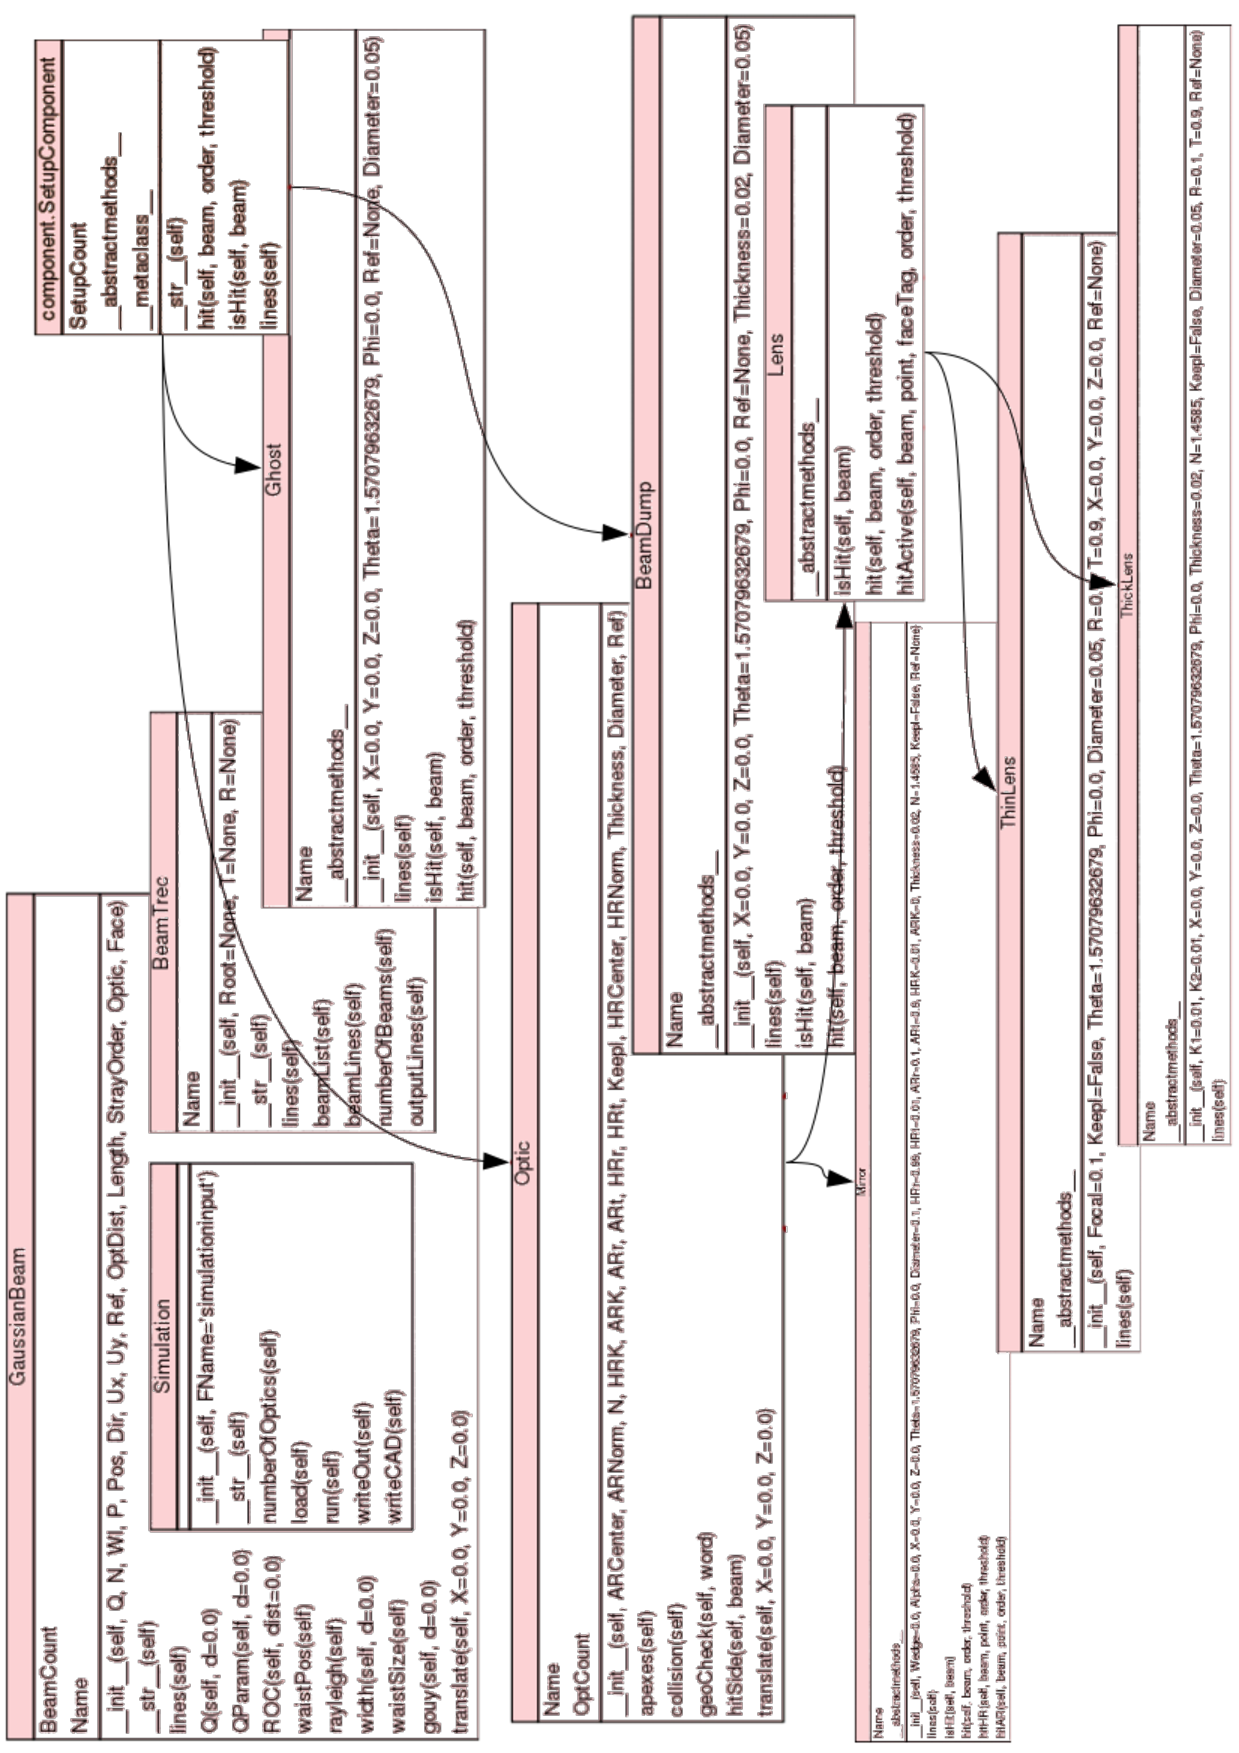
\includegraphics[scale=1]{inheritancehierarchy}
\label{inheritancehierarchy}
\end{center}
\end{figure}
\paragraph{A word on initializer default values.}We try to avoid surprises and stay consistent throughout the code with the following policies concerning classes at the leaves of the inheritance graph:

\begin{enumerate}
\item For classes whose initializers will be called only with input form users (read from an input file or in a a script), \textit{every} parameter of the constructor has a default value and the constructor can be called \textit{without arguments}. What's more, the input of the user is processed through the class initializer and then fed to the initializer of the mother class. For example, the user may provide \tt{X}, \tt{Y} and \tt{Z} to the constructor she or he calls, then these are processed and it is \tt{[X, Y, Z]} as a list (with types checked etc.) which is fed to the mother initializer. This concerns the constructors for \tt{ThinLens}, \tt{ThickLens}, \tt{Mirror}, \tt{BeamDump}.

\item For classes whose initializers are called solely internally, there are \textit{no default values}. These are the constructors of \tt{SetupComponent}, \tt{Optic}.

\item For classes that may be instantiated internally and by users, the class has a \tt{classmethod} decorated method, whose parameters \textit{all have default values} and which is intended to be used with input from the user, as the constructors described in the previous point 1. This method is named \tt{user\$CLASSNAME} and processes the input of the user into input for the class's proper \tt{\_\_init\_\_} initializer. On the other hand, this proper initializer is intended for internal use only and has \textit{no default values}. This is for example the case of the \tt{optics.beam.GaussianBeam} class, whose constructor is called internally to generate new beams and with user input read from the input file. In this last case it is \tt{userGaussianBeam} which is called.
\end{enumerate}

\paragraph{Abstract Base Classes.}The highest class of the optical classes hierarchy is the \tt{optics.component.SetupComponent} class. Its metaclass is set to \tt{abc.ABCMeta}, making it an abstract base class\footnote{See \tt{docs.python.org/2/library/abc.html} for details}. This essentially means that no daughter class of this class can be instantiated unless all the methods decorated with \tt{abc.abstractmethod} have been reimplemented by the daughter class. The methods concerned with this limitation are \tt{optics.component.SetupComponent.lines} and \tt{optics.component.SetupComponent.isHit}. Methods decorated with \tt{abstractmethod} in an abstract base class can eventually be implemented in the mother class, but in theia they all \tt{pass}, and could be called \textit{pure virtual} for someone coming from C++.
\subsection{Call graph}

Here is the call graph of the theia CLI tool, from which one can easily deduce the call graph of any individual function.


\begin{figure}[h]
\begin{center}
%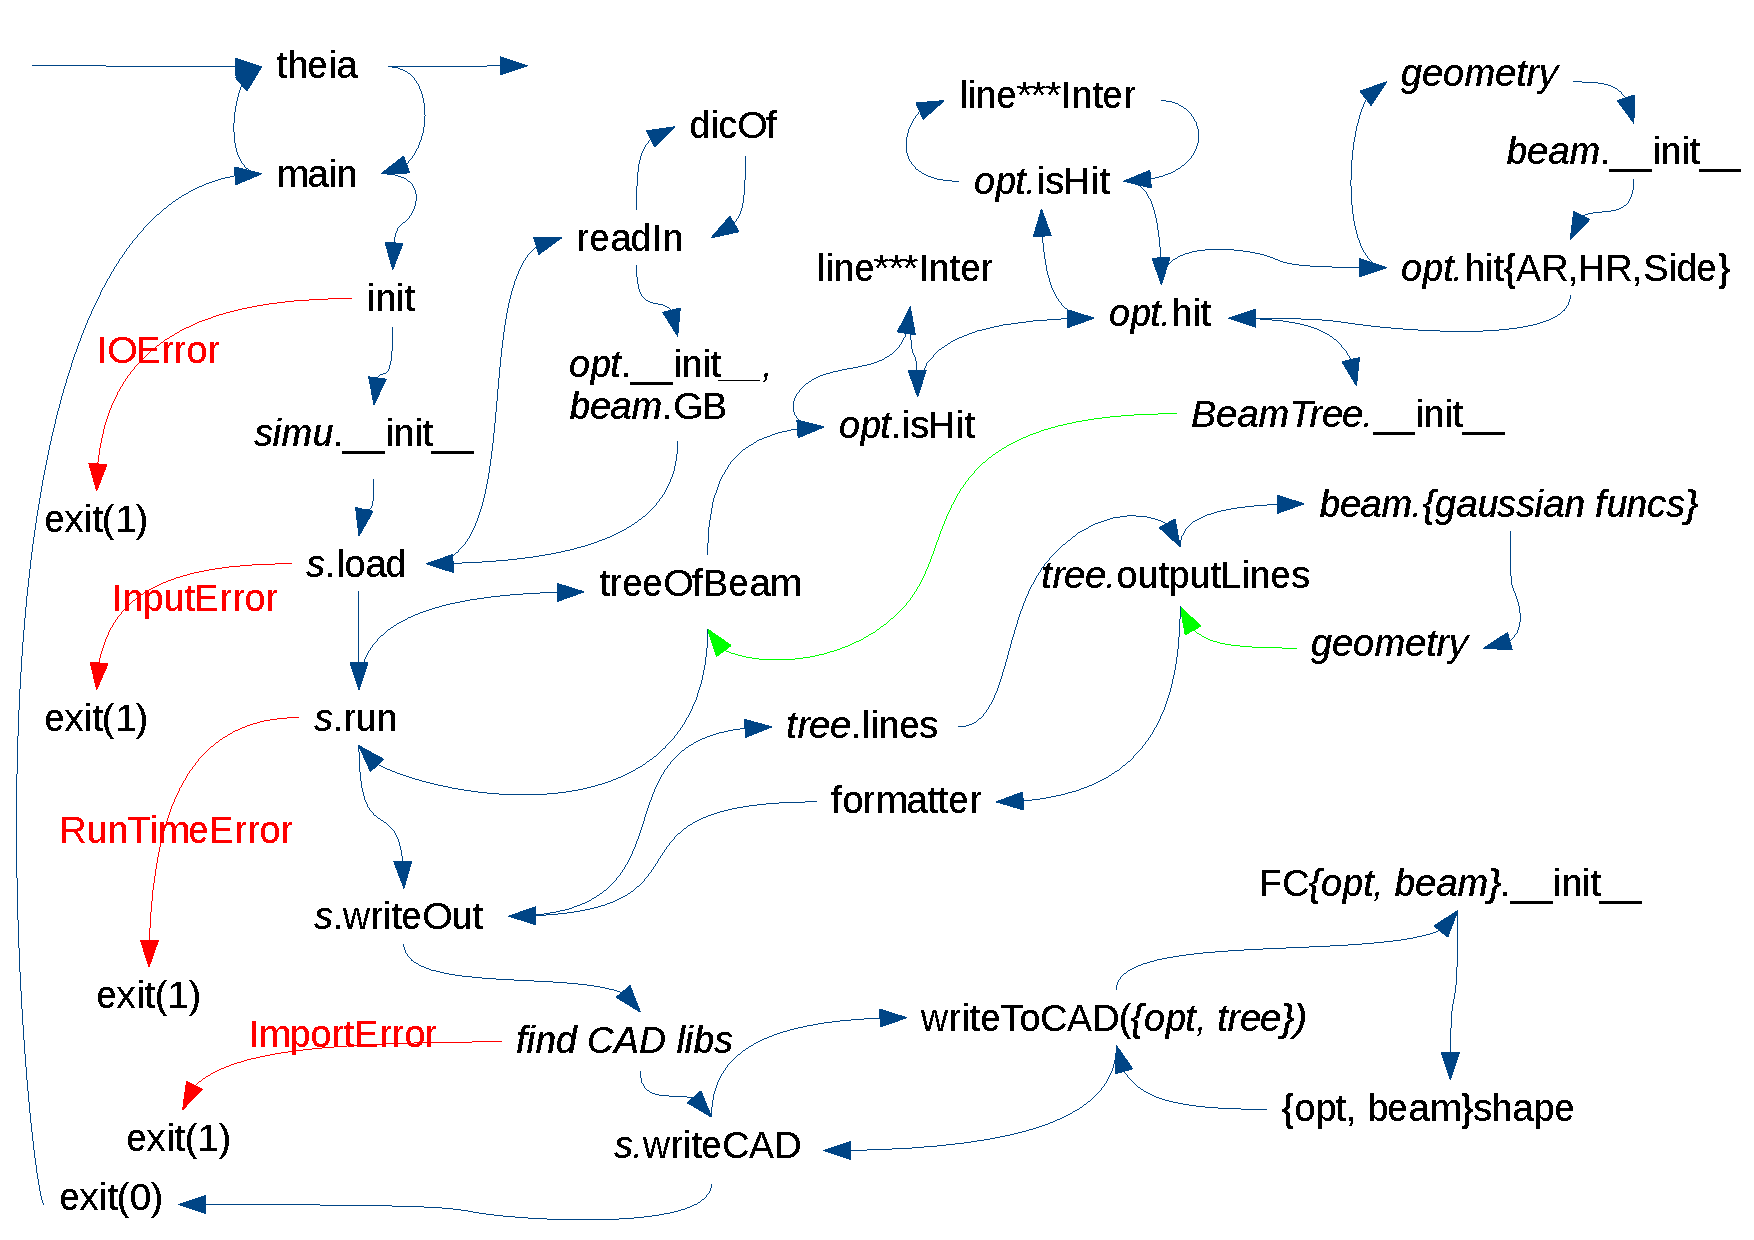
\includegraphics[scale=1]{callgraph}
\end{center}
\caption{Call graph of the theia CLI tool}
\label{callgraph}
\end{figure}

For a more concise view, here is the dependency tree of the functions of the theia library.

\begin{figure}[h]
\begin{center}
%\includegraphics[scale=1]{functiondependencies}
\end{center}
\caption{Dependencies of the functions of the theia library}
\end{figure}

\paragraph{Note on the stack.}According to this call graph (figure \ref{callgraph}), the stack has a maximum height of $9~+~2(n-1)$ when there are $n$ levels of recursion. Generally, the program crashes -- if it crashes -- by recursion depth limit exceeding (leading to a handled \tt{RunTimeError} exception and an exit with an error code of 1) before causing a stack overflow.

\subsection{Miscellaneous remarks}

\paragraph{Coding style.}In the development of theia we have tried to stick to a couple of coding style conventions, which may help to review the code and are important to know for anyone wishing to contribute.

\begin{itemize}
\item The code of theia is heavily commented and doc-stringed, and it should stay that way in order for theia to be an accessible library.

\item Throughout the library, classes and attributes look \tt{LikeThis} whereas objects and methods look \tt{likeThis}.

\item There is an approximate (it isn't true only in the \tt{helpers} sub-package) \textit{one file} $\rightarrow$ \textit{one class} correspondence and files are named accordingly with the objects they define. Generally, we have a tendency to distribute functions in different modules if they provide different functionalities, regardless of the total number of modules. Functions are together in a module if they belong together, consequently they are many modules in theia.

\item We tend never to skip more than 1 line (Python is already very formatted).

\item \tt{\# Provides} lines at the very beginning of modules allow to know at a glance what variables, functions and classes the module provides.

\item Imports: import first from the Python standard library and third-party packages, then from theia sub-packages other than the current, then from the current theia sub-package. For theia sub-packages imports, always use the \tt{from ... import} idiom, always use relative imports (\tt{from ..helpers import interaction}) and for standard library and third-parties always \tt{import} before you \tt{from ... import}. We try to not import what we don't need.

\item Class doc-string: present class attributes before instance attributes and mention if they are inherited.
\end{itemize}

\paragraph{Writing to \tt{stdout} and files.}Many classes reimplement the \tt{\_\_str\_\_} method to have \tt{print(object)} print a neatly formated description of the object. To this effect there are two important methods: \tt{lines} (instance method) and \tt{helpers.tools.formatter} (global scope function). \tt{formatter} takes a list of strings (lines to output) and makes C-style indented output with curly braces in the right place in one large string. Basically, one has:

\begin{lstlisting}
# inside class scope
def __str__(self):
	return formatter(self.lines())
	
\end{lstlisting}


\end{document} 
